\section{eo\-Mon\-Op$<$ EOType $>$ Class Template Reference}
\label{classeo_mon_op}\index{eoMonOp@{eoMonOp}}
eo\-Mon\-Op is the monary operator: genetic operator that takes only one {\bf EO}{\rm (p.\,\pageref{class_e_o})}.  


{\tt \#include $<$eo\-Op.h$>$}

Inheritance diagram for eo\-Mon\-Op$<$ EOType $>$::\begin{figure}[H]
\begin{center}
\leavevmode
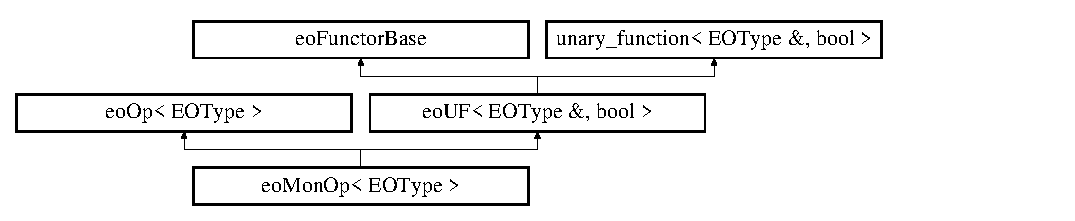
\includegraphics[height=2.52252cm]{classeo_mon_op}
\end{center}
\end{figure}
\subsection*{Public Member Functions}
\begin{CompactItemize}
\item 
{\bf eo\-Mon\-Op} ()\label{classeo_mon_op_a0}

\begin{CompactList}\small\item\em Ctor. \item\end{CompactList}\item 
virtual std::string {\bf class\-Name} () const \label{classeo_mon_op_a1}

\end{CompactItemize}


\subsection{Detailed Description}
\subsubsection*{template$<$class EOType$>$ class eo\-Mon\-Op$<$ EOType $>$}

eo\-Mon\-Op is the monary operator: genetic operator that takes only one {\bf EO}{\rm (p.\,\pageref{class_e_o})}. 

When defining your own, make sure that you return a boolean value indicating that you have changed the content. 



Definition at line 101 of file eo\-Op.h.

The documentation for this class was generated from the following file:\begin{CompactItemize}
\item 
eo\-Op.h\end{CompactItemize}
